% =====================================================================
%  Part 1: Problem and data description
% =====================================================================
\setcounter{section}{0}
\section{Problem and Data Description}
\label{sec:part1}

\subsection{Problem Formulation}
\label{sec:problem}

Each sample is one \emph{recipe web page} returned by a Google Image search for
``\texttt{<dish> recipe}''~\cite{wang2015recipe}. It provides two modalities that come from the same page:
an RGB image $x^{I}$ and the page title $x^{T}$, a short string. The label $y$ is one of $K=101$ dish classes,
the same classes as Food-101~\cite{bossard2014food} in Assignment~2. A model $f_\theta$ outputs logits in
$\R^{K}$ and is trained with the cross-entropy loss
\begin{equation}
  \mathcal{L}(\theta) = -\frac{1}{N}\sum_{n=1}^{N} \log \operatorname{softmax}\big(f_\theta(x^{I}_n, x^{T}_n)\big)_{y_n}.
\end{equation}
Unimodal models see only $x^{I}$ or only $x^{T}$.

The two modalities carry different evidence, and each fails in its own way. The image shows the
appearance of the dish, but web images include advertisements, collages, ingredient shots and photos shared
by several dishes. The title often names the dish, but it can be generic (``Recipes''), describe a derived
dish (``Apple Pie Moonshine'') or name another class. These cases are the \emph{support} and \emph{conflict}
cases that the specification asks us to analyse (section~6.11).

\subsection{Dataset}
\label{sec:dataset}

We use UPMC Food-101~\cite{wang2015recipe} through the Kaggle mirror \texttt{gianmarco96/upmcfood101}.
It contains $90{,}704$ JPEG images in the official train/test lists ($67{,}988$ / $22{,}716$) and two CSV
files with the \textbf{page title} of each image. The mirror does not contain the full page text that earlier
work used~\cite{kiela2019mmbt}, so our text modality is the title only. We use the data for research only and
do not redistribute images or titles; only code, split id lists and checkpoints are published.

\subsection{Pairs and Validity}
\label{sec:pairs}

The linking entity is the \textbf{web page}. An image and a title form a pair only when they share the file
id \texttt{<label>\_<num>}, the label and the official split; samples are never paired at random. The script
\texttt{scripts/prepare\_data.py} checks the validity criteria of the proposal (\cref{tab:validity}).
A \emph{complete pair} satisfies criteria 1--3. All models are trained, selected and tested on complete pairs.
Items whose title fails criterion~2 form the natural missing-text set.

\begin{table}[H]
  \centering\small
  \caption{Pair-validity criteria and their outcome on the full dataset.}
  \label{tab:validity}
  \begin{tabularx}{\linewidth}{@{}lYl@{}}
    \toprule
    Criterion & Rule & Result \\
    \midrule
    1. Image valid & decodes, shorter side $\ge 64$\,px, pixel standard deviation $> 2$ & $90{,}701$ / $90{,}704$ \\
    2. Text valid  & a title row exists and contains at least one content word ($\ge 3$ letters, not in a fixed list of generic web words such as \emph{recipes}, \emph{easy}, \emph{pinterest}) & $90{,}192$ / $90{,}704$ \\
    3. Same item   & same id, label and official split & all $90{,}688$ titles matched \\
    4. Manual audit & 200 train pairs, 10 from each of 20 random classes & $81.5\%$ valid (\cref{sec:audit}) \\
    \bottomrule
  \end{tabularx}
\end{table}

Of the $512$ items without a valid title, $16$ have no title row at all and $496$ fail the content-word rule.
The most frequent failing titles are ``All Yummy Recipes'', ``Recipes'', ``Recipes on Pinterest'', ``Easy'' and
``Food''. Three images are near-constant placeholders.

\subsection{Exploratory Data Analysis}
\label{sec:eda}

The EDA (\texttt{scripts/eda.py}) covers pair counts, pair quality, missing-modality rates and
modality-specific distributions, as required by section~6.10. \Cref{fig:samples} shows random training pairs.

\begin{figure}[H]
  \centering
  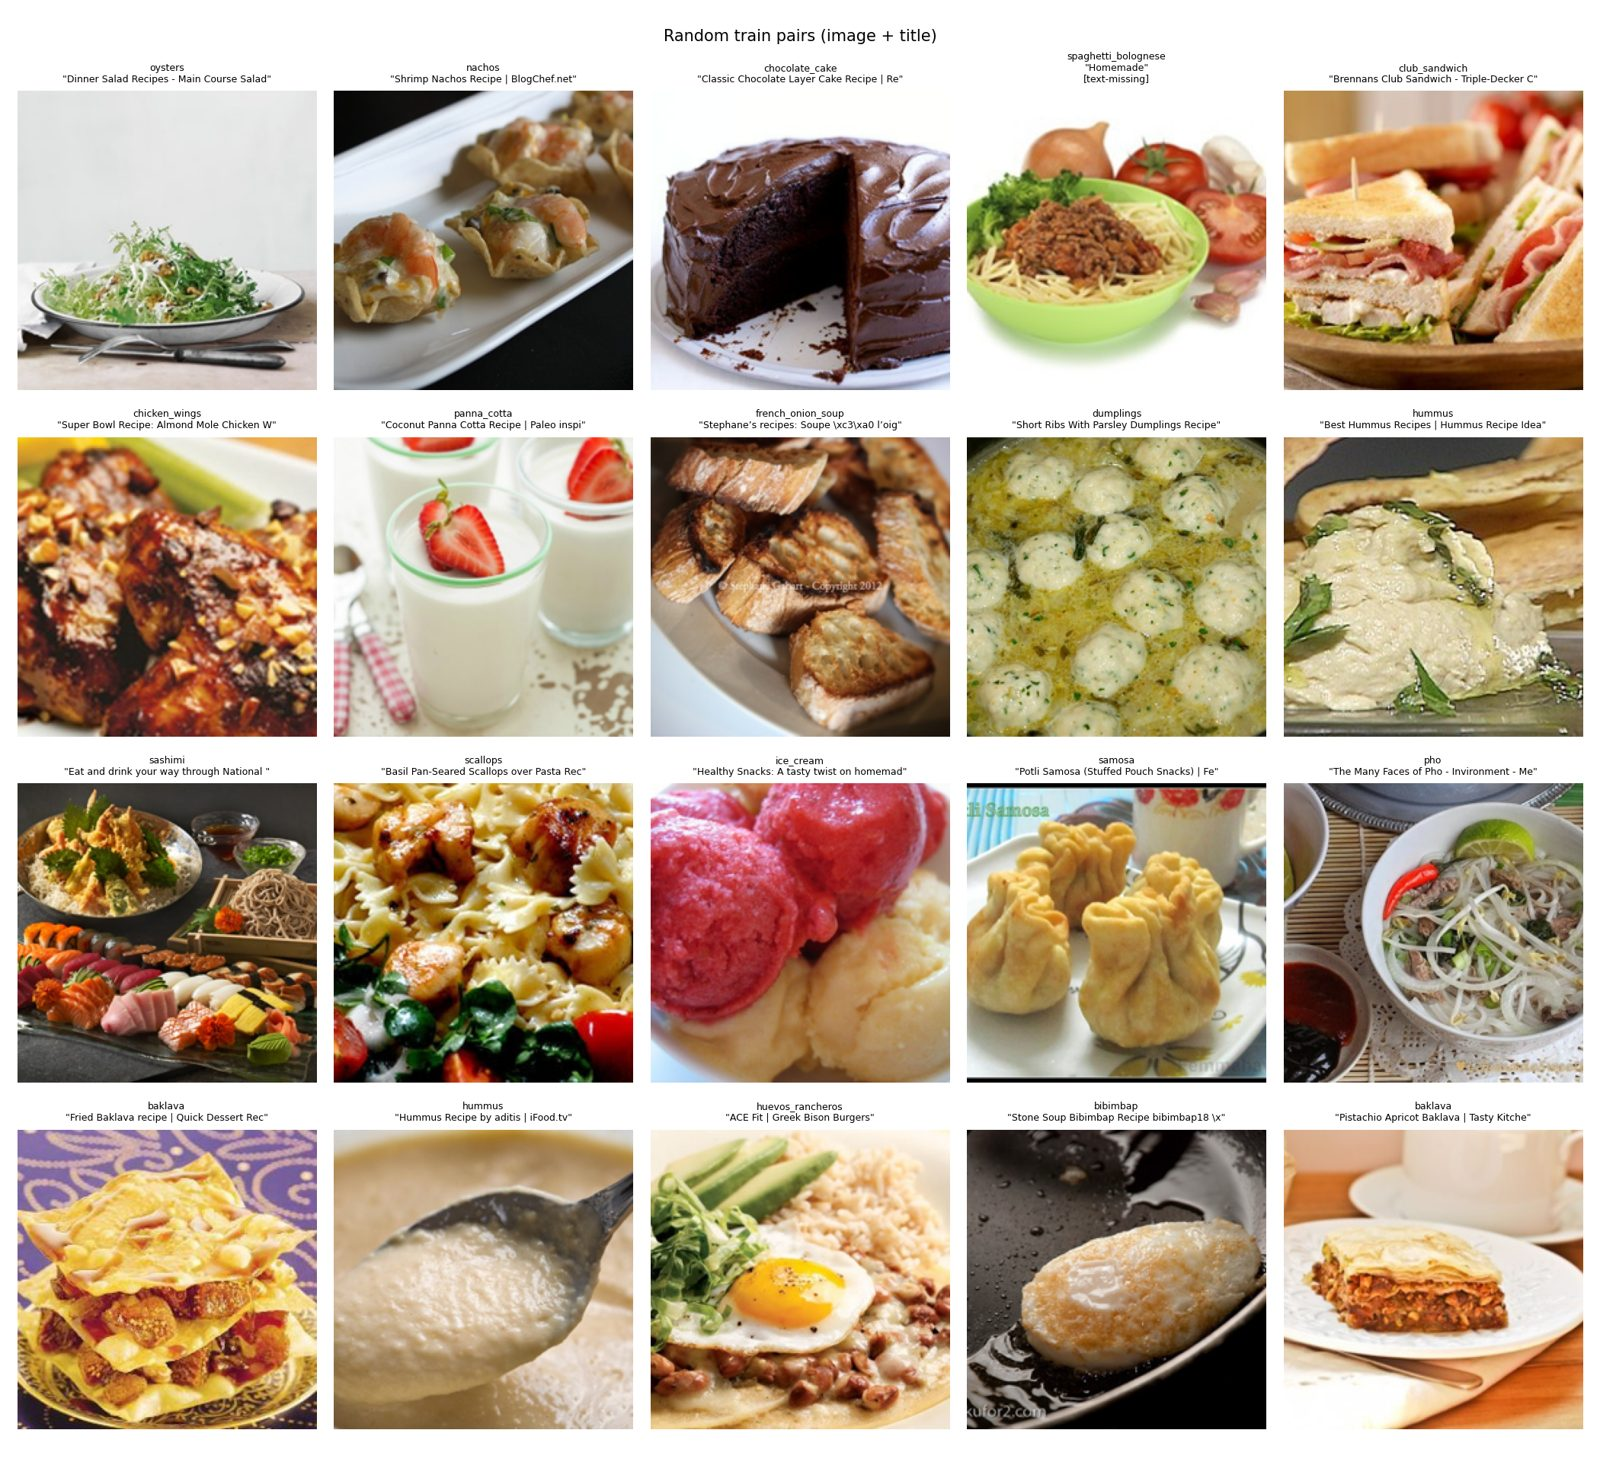
\includegraphics[width=0.95\linewidth]{samples_pairs.jpg}
  \caption{Twenty random training pairs with their class label and title. Titles are noisy web strings: site
  names, generic titles (``Homemade'' fails the validity rule), derived dishes, and pages whose title does not
  describe the image.}
  \label{fig:samples}
\end{figure}

\paragraph{Pair counts and missing modalities.}
\Cref{tab:counts} gives the counts per split. Missing modalities are rare: about $0.6\%$ of the items have an
uninformative title, and only three images are invalid. The classes are mildly imbalanced (largest/smallest
class $1.21$ in train), so macro-F1 is the primary metric. The highest text-missing rates per class are
\cls{hot\_dog} ($5.5\%$) and \cls{breakfast\_burrito} ($3.5\%$).

\begin{table}[H]
  \centering\small
  \caption{Items per split after the pair checks.}
  \label{tab:counts}
  \begin{tabular}{@{}lrrrrrr@{}}
    \toprule
    Split & Items & Complete pairs & Text-missing & Image-missing & Train duplicate & Cross-label cluster \\
    \midrule
    train & $63{,}128$ & $\mathbf{62{,}771}$ & $355$ & $2$ & -- & $869$ \\
    val   & $4{,}860$  & $\mathbf{4{,}824}$  & $36$  & $0$ & -- & $75$ \\
    test  & $22{,}716$ & $\mathbf{22{,}594}$ & $121$ & $1$ & $3{,}290$ ($14.5\%$) & $296$ \\
    \bottomrule
  \end{tabular}
\end{table}

\paragraph{Label information in the title.}
The search query leaked the class name into most titles. We match titles against a class-name lexicon
(names, singular and plural forms, and 82 hand-written synonyms for 50 classes, fixed from the class list and
train titles only). \Cref{tab:mention} summarises the results. A keyword rule that predicts the most-mentioned
class (K0) already reaches $76.8\%$ test accuracy without any learning. The share of titles that name their
own class ranges from $7\%$ (\cls{hot\_dog}) and $30\%$ (\cls{beef\_tartare}) to $97.5\%$ (\cls{pancakes}),
see \cref{fig:mention}.

\begin{table}[H]
  \centering\small
  \caption{Class names in titles (complete pairs).}
  \label{tab:mention}
  \begin{tabular}{@{}lrrrrr@{}}
    \toprule
    Split & Own class, exact & Own class, lexicon & Another class only & No class & K0 accuracy \\
    \midrule
    train & $72.3\%$ & $78.8\%$ & $1.0\%$ & $20.2\%$ & $76.9\%$ \\
    test  & $72.4\%$ & $78.8\%$ & $0.9\%$ & $20.2\%$ & $76.8\%$ \\
    \bottomrule
  \end{tabular}
\end{table}

\begin{figure}[H]
  \centering
  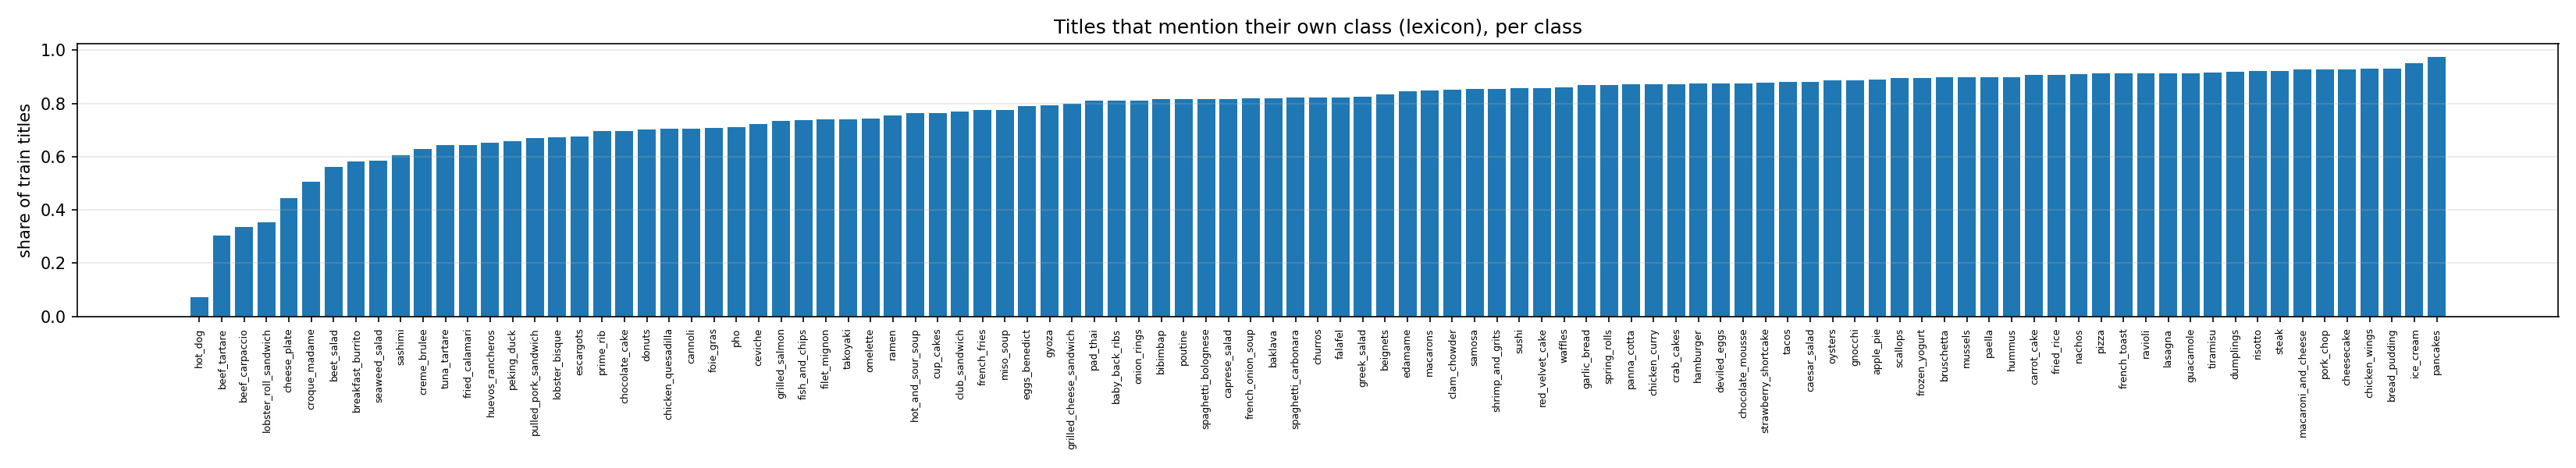
\includegraphics[width=\linewidth]{class_name_mention_per_class.png}
  \caption{Share of train titles that mention their own class, per class (sorted).}
  \label{fig:mention}
\end{figure}

\paragraph{Text distributions.}
Titles are short: the median is $7$ words and $13$ DistilBERT tokens, the 99th percentile $39$ tokens. Only
$126$ titles ($0.14\%$) exceed the $64$-token limit (\cref{fig:text}). The train vocabulary has $29{,}847$
lower-cased words.
\begin{itemize}
  \item \textbf{Site names.} $64\%$ of the titles end with a site segment (``| Taste of Home'', ``on Pinterest'').
        For the $96$ sites with at least $50$ train items, the majority class covers only $16\%$ of a site's
        items on average, so the site name alone is a weak class cue.
  \item \textbf{Encoding errors.} Some titles contain literally escaped UTF-8 bytes
        (``Soupe \textbackslash xc3\textbackslash xa0 l'oig'') or JSON-like brackets. These are crawl errors
        that we keep as they are.
\end{itemize}

\begin{figure}[H]
  \centering
  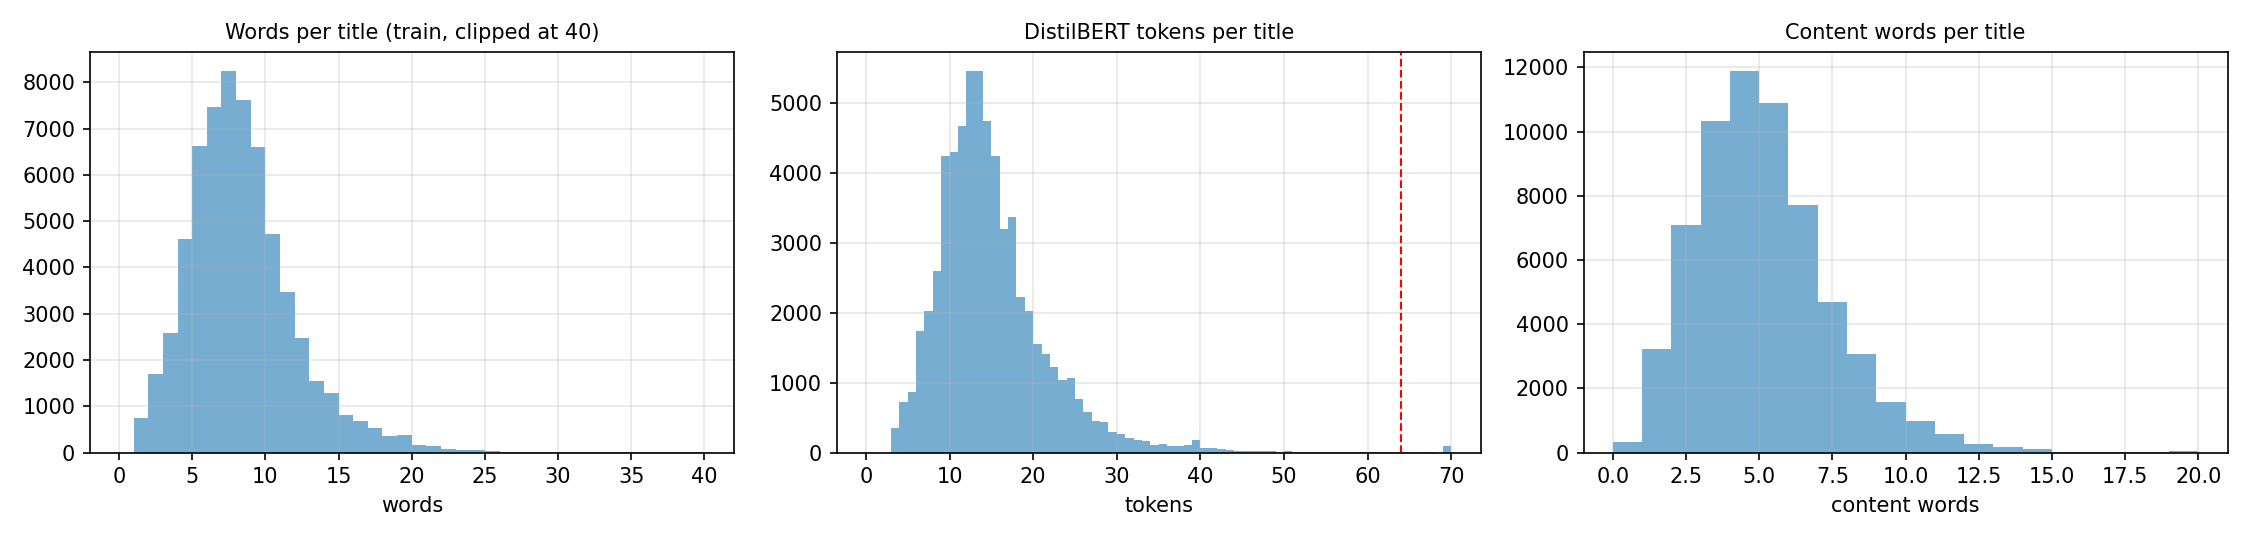
\includegraphics[width=\linewidth]{text_lengths.png}
  \caption{Words, DistilBERT tokens and content words per train title. The red line marks the 64-token limit.}
  \label{fig:text}
\end{figure}

\paragraph{Image distributions.}
The images are web photos of varied geometry (\cref{fig:images}).
\begin{itemize}
  \item Shorter side: median $387$\,px, range $120$--$900$\,px.
  \item Aspect ratio: median $1.33$, range $0.09$--$8.73$. The extreme values are banners and collages.
  \item The training mean colour $[0.628, 0.529, 0.422]$ is brighter than ImageNet's $[0.485, 0.456, 0.406]$
        because many recipe sites use white backgrounds. The pretrained encoders still use the ImageNet
        statistics they were trained with.
\end{itemize}
We store a copy resized to a shorter side of $256$\,px, which keeps all the detail used at $224$\,px.

\begin{figure}[H]
  \centering
  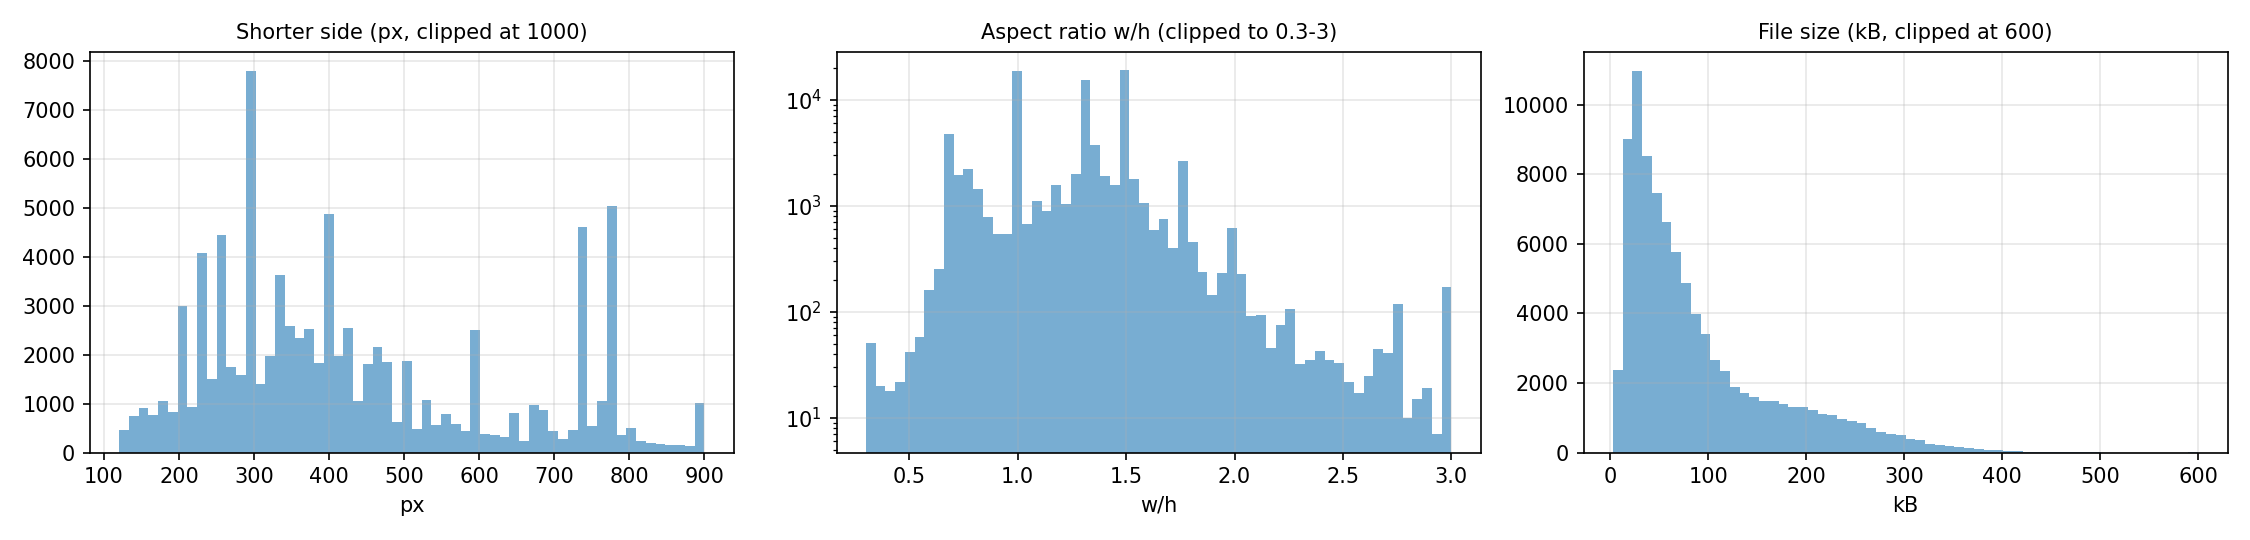
\includegraphics[width=\linewidth]{image_stats.png}
  \caption{Shorter side, aspect ratio and file size of all images.}
  \label{fig:images}
\end{figure}

\paragraph{Duplicates.}
We link two items when their files are identical (md5) or when their 64-bit perceptual hashes~\cite{zauner2010phash}
differ by at most $4$ bits.
\begin{itemize}
  \item There are $3{,}597$ md5 links and $12{,}663$ pHash pairs. Their connected components form $7{,}201$
        clusters with at least two items ($16{,}498$ items; the largest cluster has $16$).
  \item $524$ clusters carry two or more labels (\cref{fig:dups}), which is label noise built into the crawl.
  \item $3{,}290$ test items ($14.5\%$) are linked to an image in the official train list.
  \item Independently of the images, $10{,}859$ normalised titles occur more than once, $4{,}873$ of them in
        both official lists.
\end{itemize}

\begin{figure}[H]
  \centering
  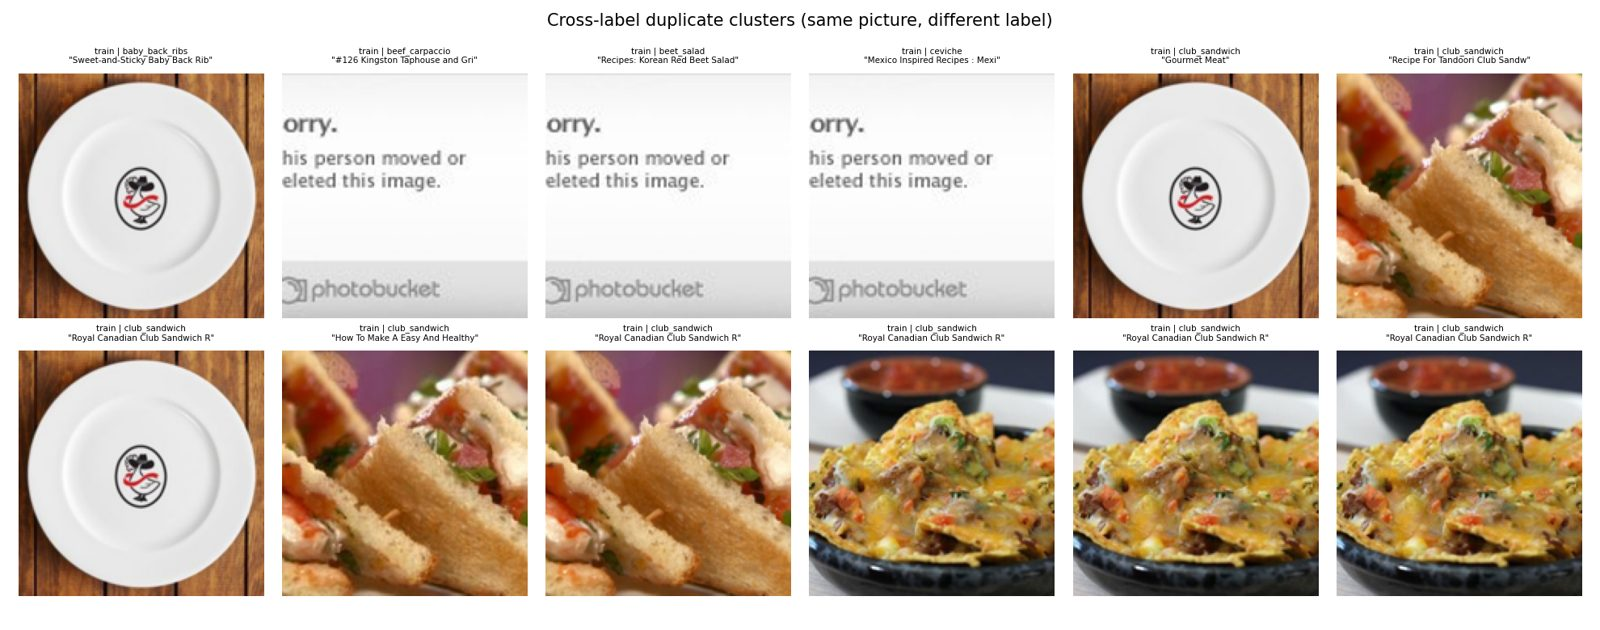
\includegraphics[width=0.9\linewidth]{duplicates_cross_label.jpg}
  \caption{Cross-label duplicate clusters: the same picture appears under different classes.}
  \label{fig:dups}
\end{figure}

\subsection{Pair Audit}
\label{sec:audit}

Ten random train pairs were drawn from each of 20 random classes (seed $42$) and labelled by hand with
\texttt{scripts/audit\_pairs.py}: Phan Bá Thanh labelled pairs 1--100 and Trần Công Hoàng Phước pairs 101--200.
Each pair is classified as \emph{valid}, \emph{image unrelated}, \emph{text unrelated}, \emph{both unrelated},
or \emph{wrong label} (image and title agree with each other but not with the class). Rates are reported with
Wilson $95\%$ confidence intervals~\cite{wilson1927}.

\begin{table}[H]
  \centering\small
  \caption{Manual audit of 200 train pairs (\texttt{data/audit/pair\_audit.csv}).}
  \label{tab:audit}
  \begin{tabular}{@{}lrrl@{}}
    \toprule
    Verdict & Count & Rate & Wilson 95\% CI \\
    \midrule
    valid           & $163$ & $\mathbf{81.5\%}$ & $75.5$--$86.3\%$ \\
    image unrelated & $16$  & $8.0\%$  & $5.0$--$12.6\%$ \\
    text unrelated  & $17$  & $8.5\%$  & $5.4$--$13.2\%$ \\
    both unrelated  & $3$   & $1.5\%$  & $0.5$--$4.3\%$ \\
    wrong label     & $1$   & $0.5\%$  & $0.1$--$2.8\%$ \\
    \midrule
    \textit{image uninformative (image + both)} & $19$ & $9.5\%$  & $6.2$--$14.4\%$ \\
    \textit{title uninformative (text + both)}  & $20$ & $10.0\%$ & $6.6$--$14.9\%$ \\
    \bottomrule
  \end{tabular}
\end{table}

\begin{itemize}
  \item \textbf{One pair in five is noisy, and usually in one modality only.} Only $1.5\%$ of the pairs are
        unrelated in both modalities. When one side is uninformative, the other usually still carries the class.
        These pairs are the raw material of the conflict groups (\cref{sec:support}).
  \item \textbf{The noise is concentrated in a few classes:}
        \begin{itemize}
          \item \cls{peking\_duck}: 5 of its 10 images are unrelated;
          \item \cls{grilled\_salmon}: 5 of its 10 titles are unrelated;
          \item \cls{hot\_and\_sour\_soup}: 4 of its 10 titles are unrelated;
          \item seven of the 20 classes have no noisy pair at all.
        \end{itemize}
  \item \textbf{The automatic text rule is lenient.} Criterion~2 flags only 2 of the 20 titles judged
        uninformative. It catches empty or generic titles, but not the titles of other pages or recipes.
        The real share of uninformative titles is therefore about $10\%$, not the $0.6\%$ text-missing rate of
        \cref{tab:counts}, and the natural missing-text set understates real missingness. A missing class name is
        a strong but not sufficient signal of a useless title: 19 of the 20 uninformative titles do not mention
        the class, against 19 of the 180 informative ones.
  \item \textbf{Wrong labels are rare ($0.5\%$).} The ETHZ Food-101 train set of Assignment~2 had $6.7\%$. Here the
        image and the title come from the same query page, so they rarely agree on a different dish. The
        cross-label duplicate clusters are the main source of label noise.
  \item \textbf{Limitations.} Each pair was judged by one rater, so there is no inter-rater agreement. The sample
        covers 20 of the 101 classes.
\end{itemize}

\subsection{Data Splitting and Leakage Prevention}
\label{sec:split}

\begin{itemize}
  \item \textbf{Split unit.} The item (one web page) is the split unit, so an image and its title can never fall into
        different splits (specification, section~6.4).
  \item \textbf{Validation.} The official train list is split by
        \texttt{StratifiedGroupKFold}~\cite{pedregosa2011sklearn} with $14 = \mathrm{round}(67{,}988/5{,}000)$ folds,
        shuffling and seed $42$. Class is the stratum and the image-duplicate cluster is the group; fold~0 is the
        validation set ($4{,}860$ items). The code asserts that no cluster is shared by train and validation.
  \item \textbf{Test.} The official test list is kept unchanged for comparability, so test items with a train
        duplicate cannot be moved. Instead, every test metric is reported again on a \textbf{dedup} subset
        ($19{,}270$ complete pairs without a train-linked image and without cross-label clusters).
  \item \textbf{Title leakage (found in M2).} $39.4\%$ of the complete test pairs ($8{,}893$) have a normalised
        title that also occurs in train or validation. Either several images of one page were split across the
        official lists, or the title is generic. The image clusters cannot see these links, so we add a third
        view: the $13{,}701$ \textbf{title-unseen} test items (\cref{sec:leakage}).
  \item \textbf{Train-only statistics.} The lexicon and the generic-word list use train information only; the image
        models use the ImageNet statistics.
  \item \textbf{Committed files.} The split is committed as \texttt{data/splits/\{train,val,test\}.csv} with
        truncated SHA-256 fingerprints in \texttt{split.json}. Every run checks these fingerprints.
\end{itemize}
